\chapter{System architecture}
The overall system is based on the client-server architectural pattern. Clients can contact the server (e.g. to join or create rooms) using the following REST protocol.

Clients can create or join rooms contacting the gameserver. When a client is inside a room it 

The main components of the server architecture are shown in figure \ref{fig:server_classes}. 

\begin{figure}[H]
	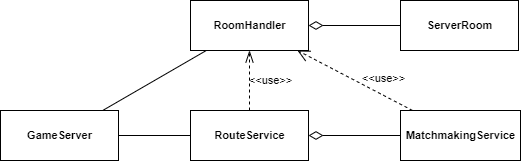
\includegraphics[scale=0.7]{images/3-architecture/server_architecture-classes.png}
	\caption{Server components class diagram}
	\label{fig:server_classes}
\end{figure}

The GameServer is the entity that listen for client requests and allows the server side developer to define new type of rooms that will be used in the application.


The RouteService is used by the gameserver to define what requests are allowed and also how to handle them. All the requests from client about rooms (e.g join, create...) are 